\feladatszam Adott az $x_2^2=x_1+3$ parabola. A parabola az $(x_1,x_2)$ síkot két tartományra osztja. Tekintse azt a tartományt, amely az origót tartalmazza. Határozza meg a tartomány azon pontjait, amelyeknél az $f(x_1,x_2)=x_1x_2$ függvény értéke a legkisebb! A megoldást az alábbi lépésekben végezze el:
\begin{alphanumericlist}
\item Írja fel az optimalizációs feladatot matematikai formában!
\item Határozza meg az összes KKT pontot!
\item Döntse el, hogy az egyes KKT pontok közül melyik lokális minimumpont!
\item Határozza meg a globális minimumpontot!
\end{alphanumericlist}

\begin{megoldas}
Először is célszerű készíteni egy ábrát a paraboláról.
\begin{center}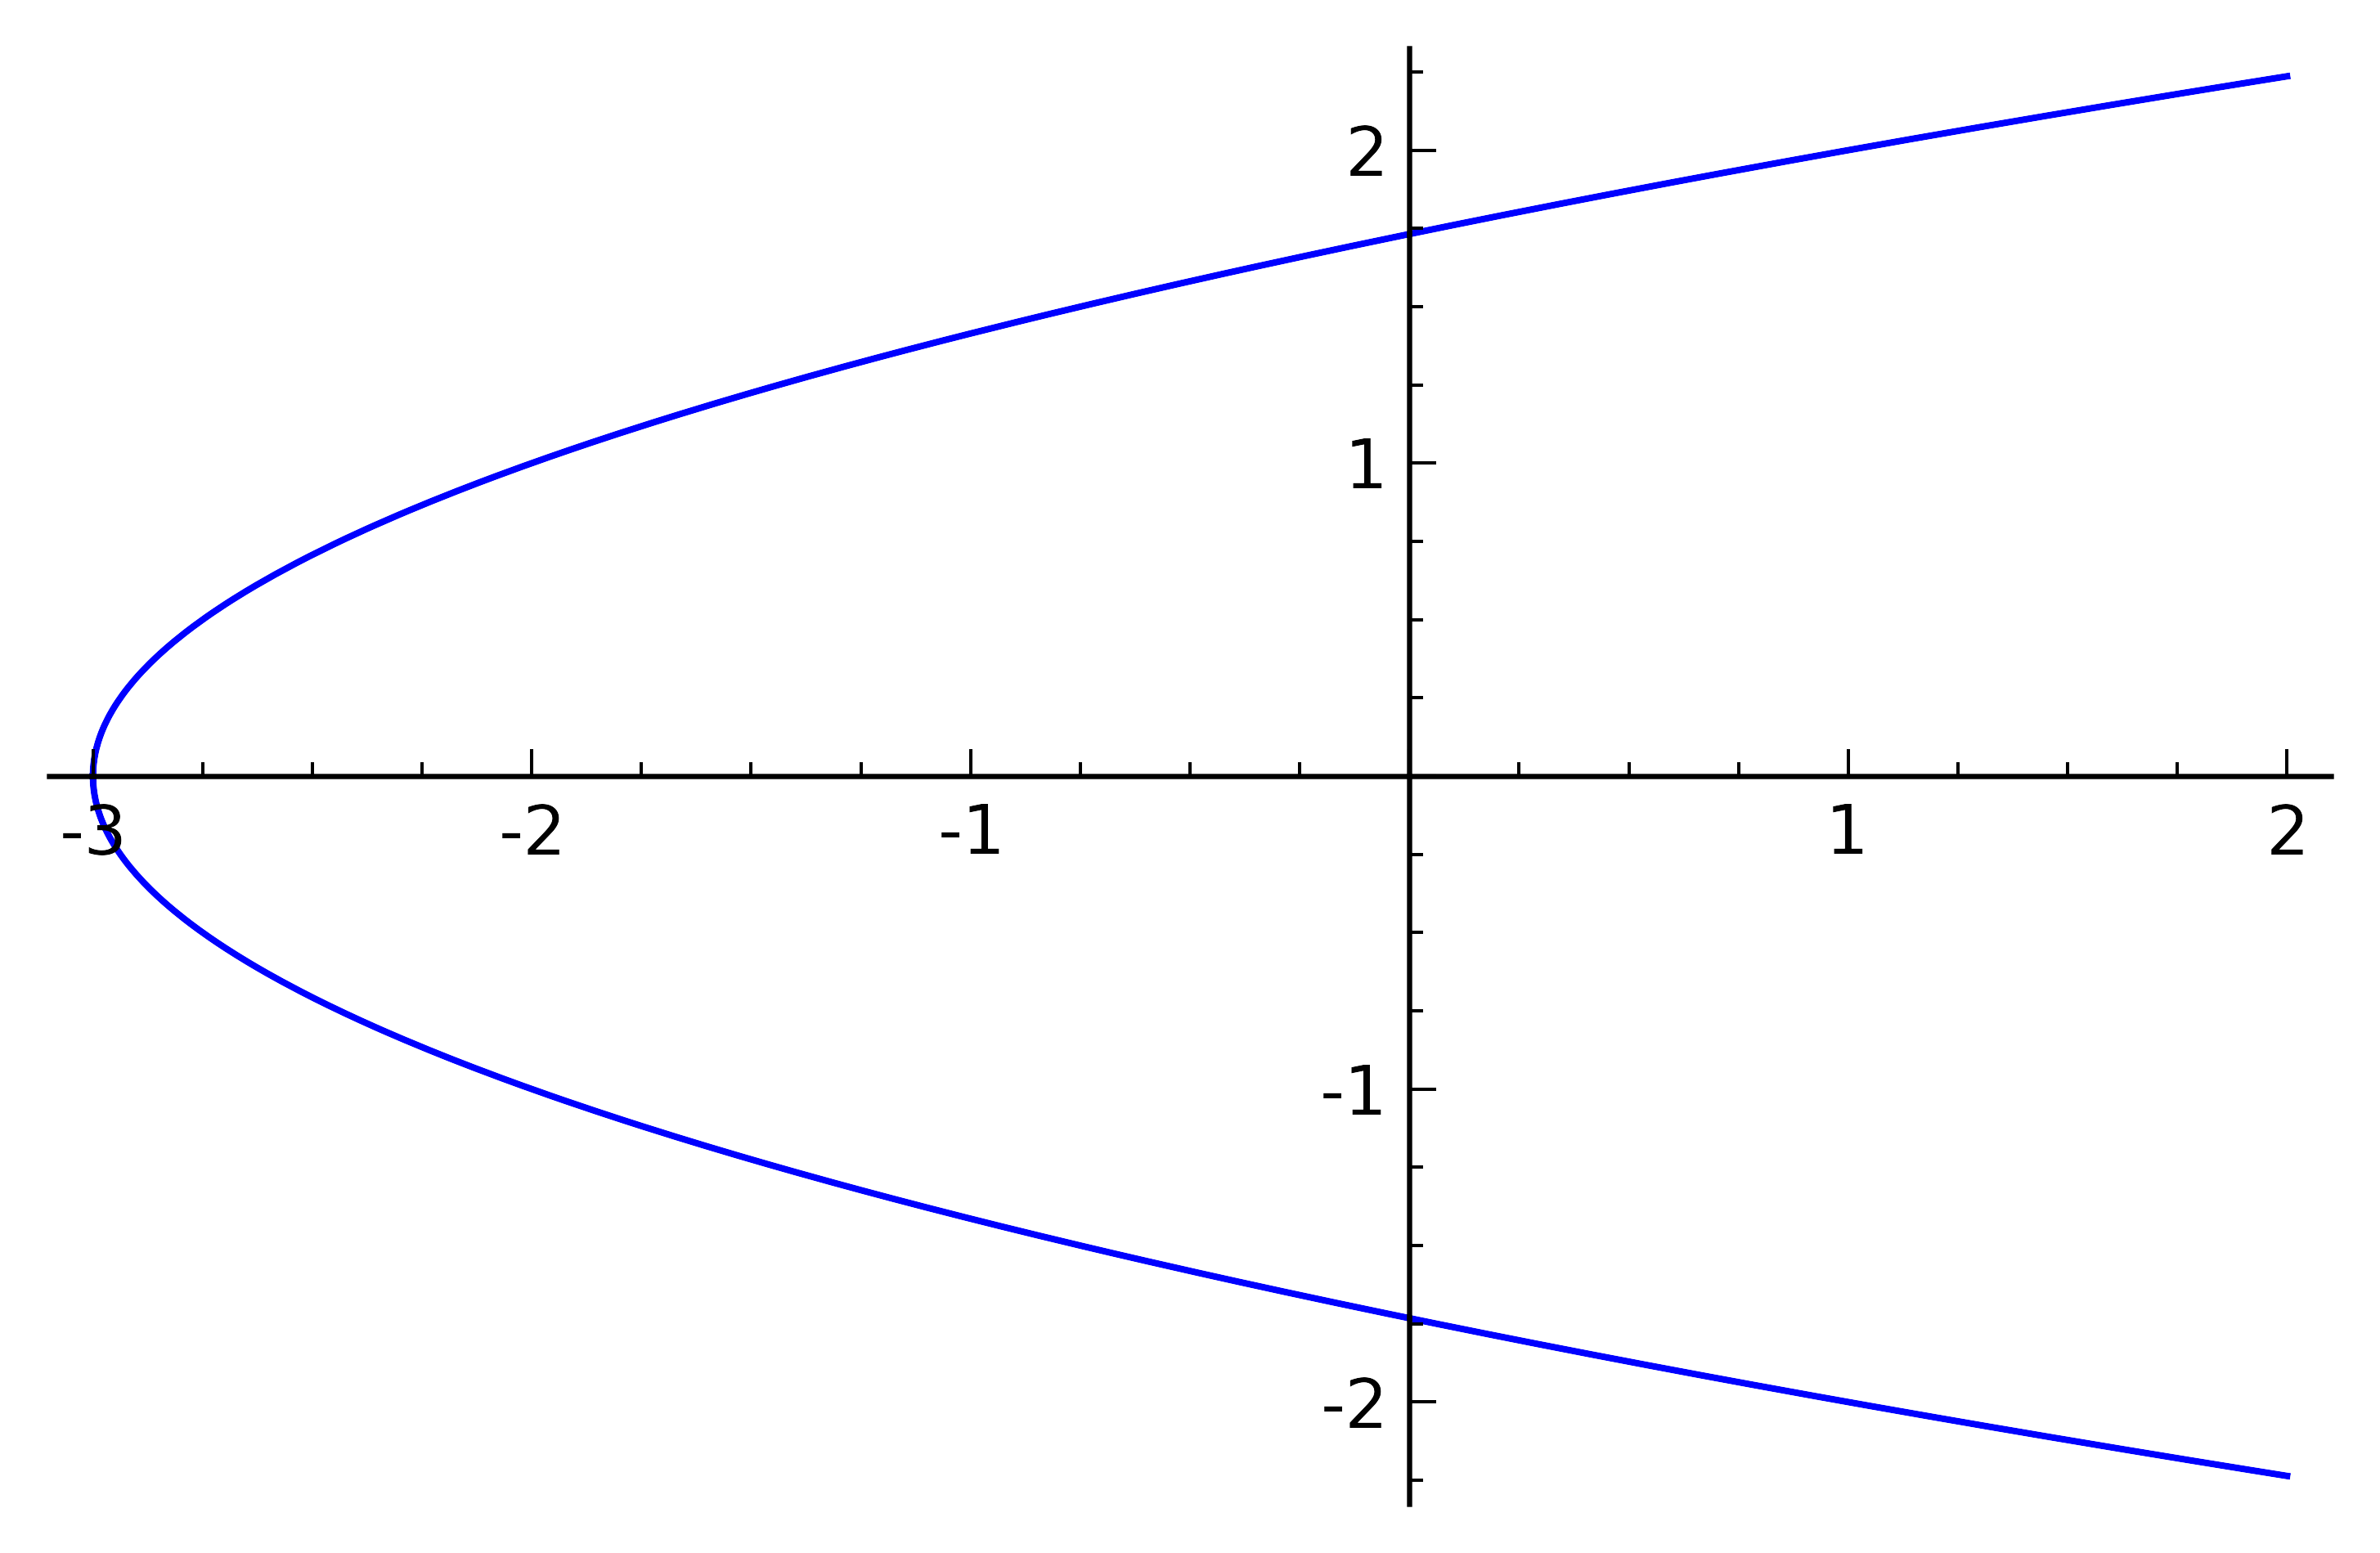
\includegraphics[scale=0.65]{kepek/kktparabola.png}\end{center}

A feladat matematikailag megfogalmazva a következő:
\begin{alignat*}{2}
x_2^2-x_1-3\leq0\\
x_1x_2\longrightarrow\min!
\end{alignat*}
\end{megoldas}

\begin{megoldas}
Most már kiszámolhatjuk a Lagrange függvényt és gradienseit:
\begin{gather*}
L(x_1,x_2,u_1,u_2)=x_1x_2+u_1(x_2^2-x_1-3)\\
\nabla L=\left(\begin{array}{c}x_2-u_1\\x_1+2x_2u_1\\\hdashline x_2^2-x_1-3\end{array}\right)\quad H=\nabla^2L=\left(\begin{array}{cc:c}0&1&-1\\1&2u_1&2x_2\\\hdashline-1&2x_2&0\end{array}\right)
\end{gather*}

A KKT feltételeket kiolvasva:
\begin{alignat*}{2}
    \left.\begin{aligned}
      x_2-u_1&=0\\
      x_1+2x_2u_1&=0
    \end{aligned}\right\} &\mbox{ duális feltételek}\\
u_1(x_2^2-x_1-3)=0\hskip 0.27cm &\mbox{ komplementaritási feltétel}\\
    \left.\begin{aligned}
      x_2^2-x_1-3&\leq0\\
      u_1&\geq0
    \end{aligned}\right\} &\mbox{ primál feltételek} 
\end{alignat*}

Esetszétválasztás:

\textbf{I. eset}: $u_1=0$
\begin{alignat*}{2}
x_2&=0\\
x_1&=0
\end{alignat*}

Ez teljesíti is a KKT feltételeket (azaz KKT pont), nézzük meg a H definitását!
\begin{gather*}
\underbrace{
\left|\begin{array}{ccc}0&\circled{1}&-1\\1&0&0\\-1&0&0\end{array}\right|\sim
\left|\begin{array}{cc}\circled{1}&0\\-1&0\end{array}\right|}_\text{Iner(1,0,1)}
\sim\underbrace{\left|\begin{array}{c}0\end{array}\right|}_\text{Iner(0,1,0)}
\end{gather*}

Az inercia értéke $\mbox{Iner}(1,1,1)$, tehát a mátrix indefinit, így az $\mathbf{x}=(0,0)^T$ csak nyeregpont.

\textbf{II. eset}: $u_1>0$
\begin{alignat*}{2}
x_2&=u_1\\
x_1+2x_2u_1&=0\\
x_2^2-x_1-3&=0
\end{alignat*}

A második egyenletbe az elsőt behelyettesítve: $x_1=-2u_1^2$. Ezt és az első egyenletet a harmadikba behelyettesítve: $u_1^2+2u_1^2-3=0$ azaz $u_1^2=1$. Ez tehát két megoldást is szolgáltat:
\begin{alignat*}{4}
u_1&=1&\quad&u_1&=-1\\
x_1&=-2&&x_1&=-2\\
x_2&=1&&x_2&=-1
\end{alignat*}

Mindkettő KKT pontot szolgáltat, a Hesse-féle mátrix definitségét vizsgálni kell:
\end{megoldas}

\begin{megoldas}
\begin{gather*}
\underbrace{\left|\begin{array}{ccc}0&1&-1\\1&\circled{$2$}&2\\-1&2&0\end{array}\right|}_\text{Iner(0,0,1)}\sim
\underbrace{\left|\begin{array}{cc}\circled{$-\nicefrac{1}{2}$}&-2\\-2&-2\end{array}\right|}_\text{Iner(1,0,0)}
\sim\underbrace{\left|\begin{array}{c}6\end{array}\right|}_\text{Iner(0,0,1)}\\
\underbrace{\left|\begin{array}{ccc}0&1&-1\\1&\circled{$-2$}&-2\\-1&-2&0\end{array}\right|}_\text{Iner(1,0,0)}\sim
\underbrace{\left|\begin{array}{cc}\circled{$\nicefrac{1}{2}$}&-2\\-2&-2\end{array}\right|}_\text{Iner(0,0,1)}
\sim\underbrace{\left|\begin{array}{c}-10\end{array}\right|}_\text{Iner(1,0,0)}
\end{gather*}

Az $\mathbf{x}=(-2,1)^T$ KKT ponthoz tartozó Hesse-féle mátrix feltételesen pozitív definit, míg az $\mathbf{x}=(-2,-1)^T$ KKT ponthoz tartozó feltételesen negatív definit. Tehát az első pont lokális minimum, a második pedig lokális maximum pont. A következő kontúrrajzon ez jól látszik:
\begin{center}
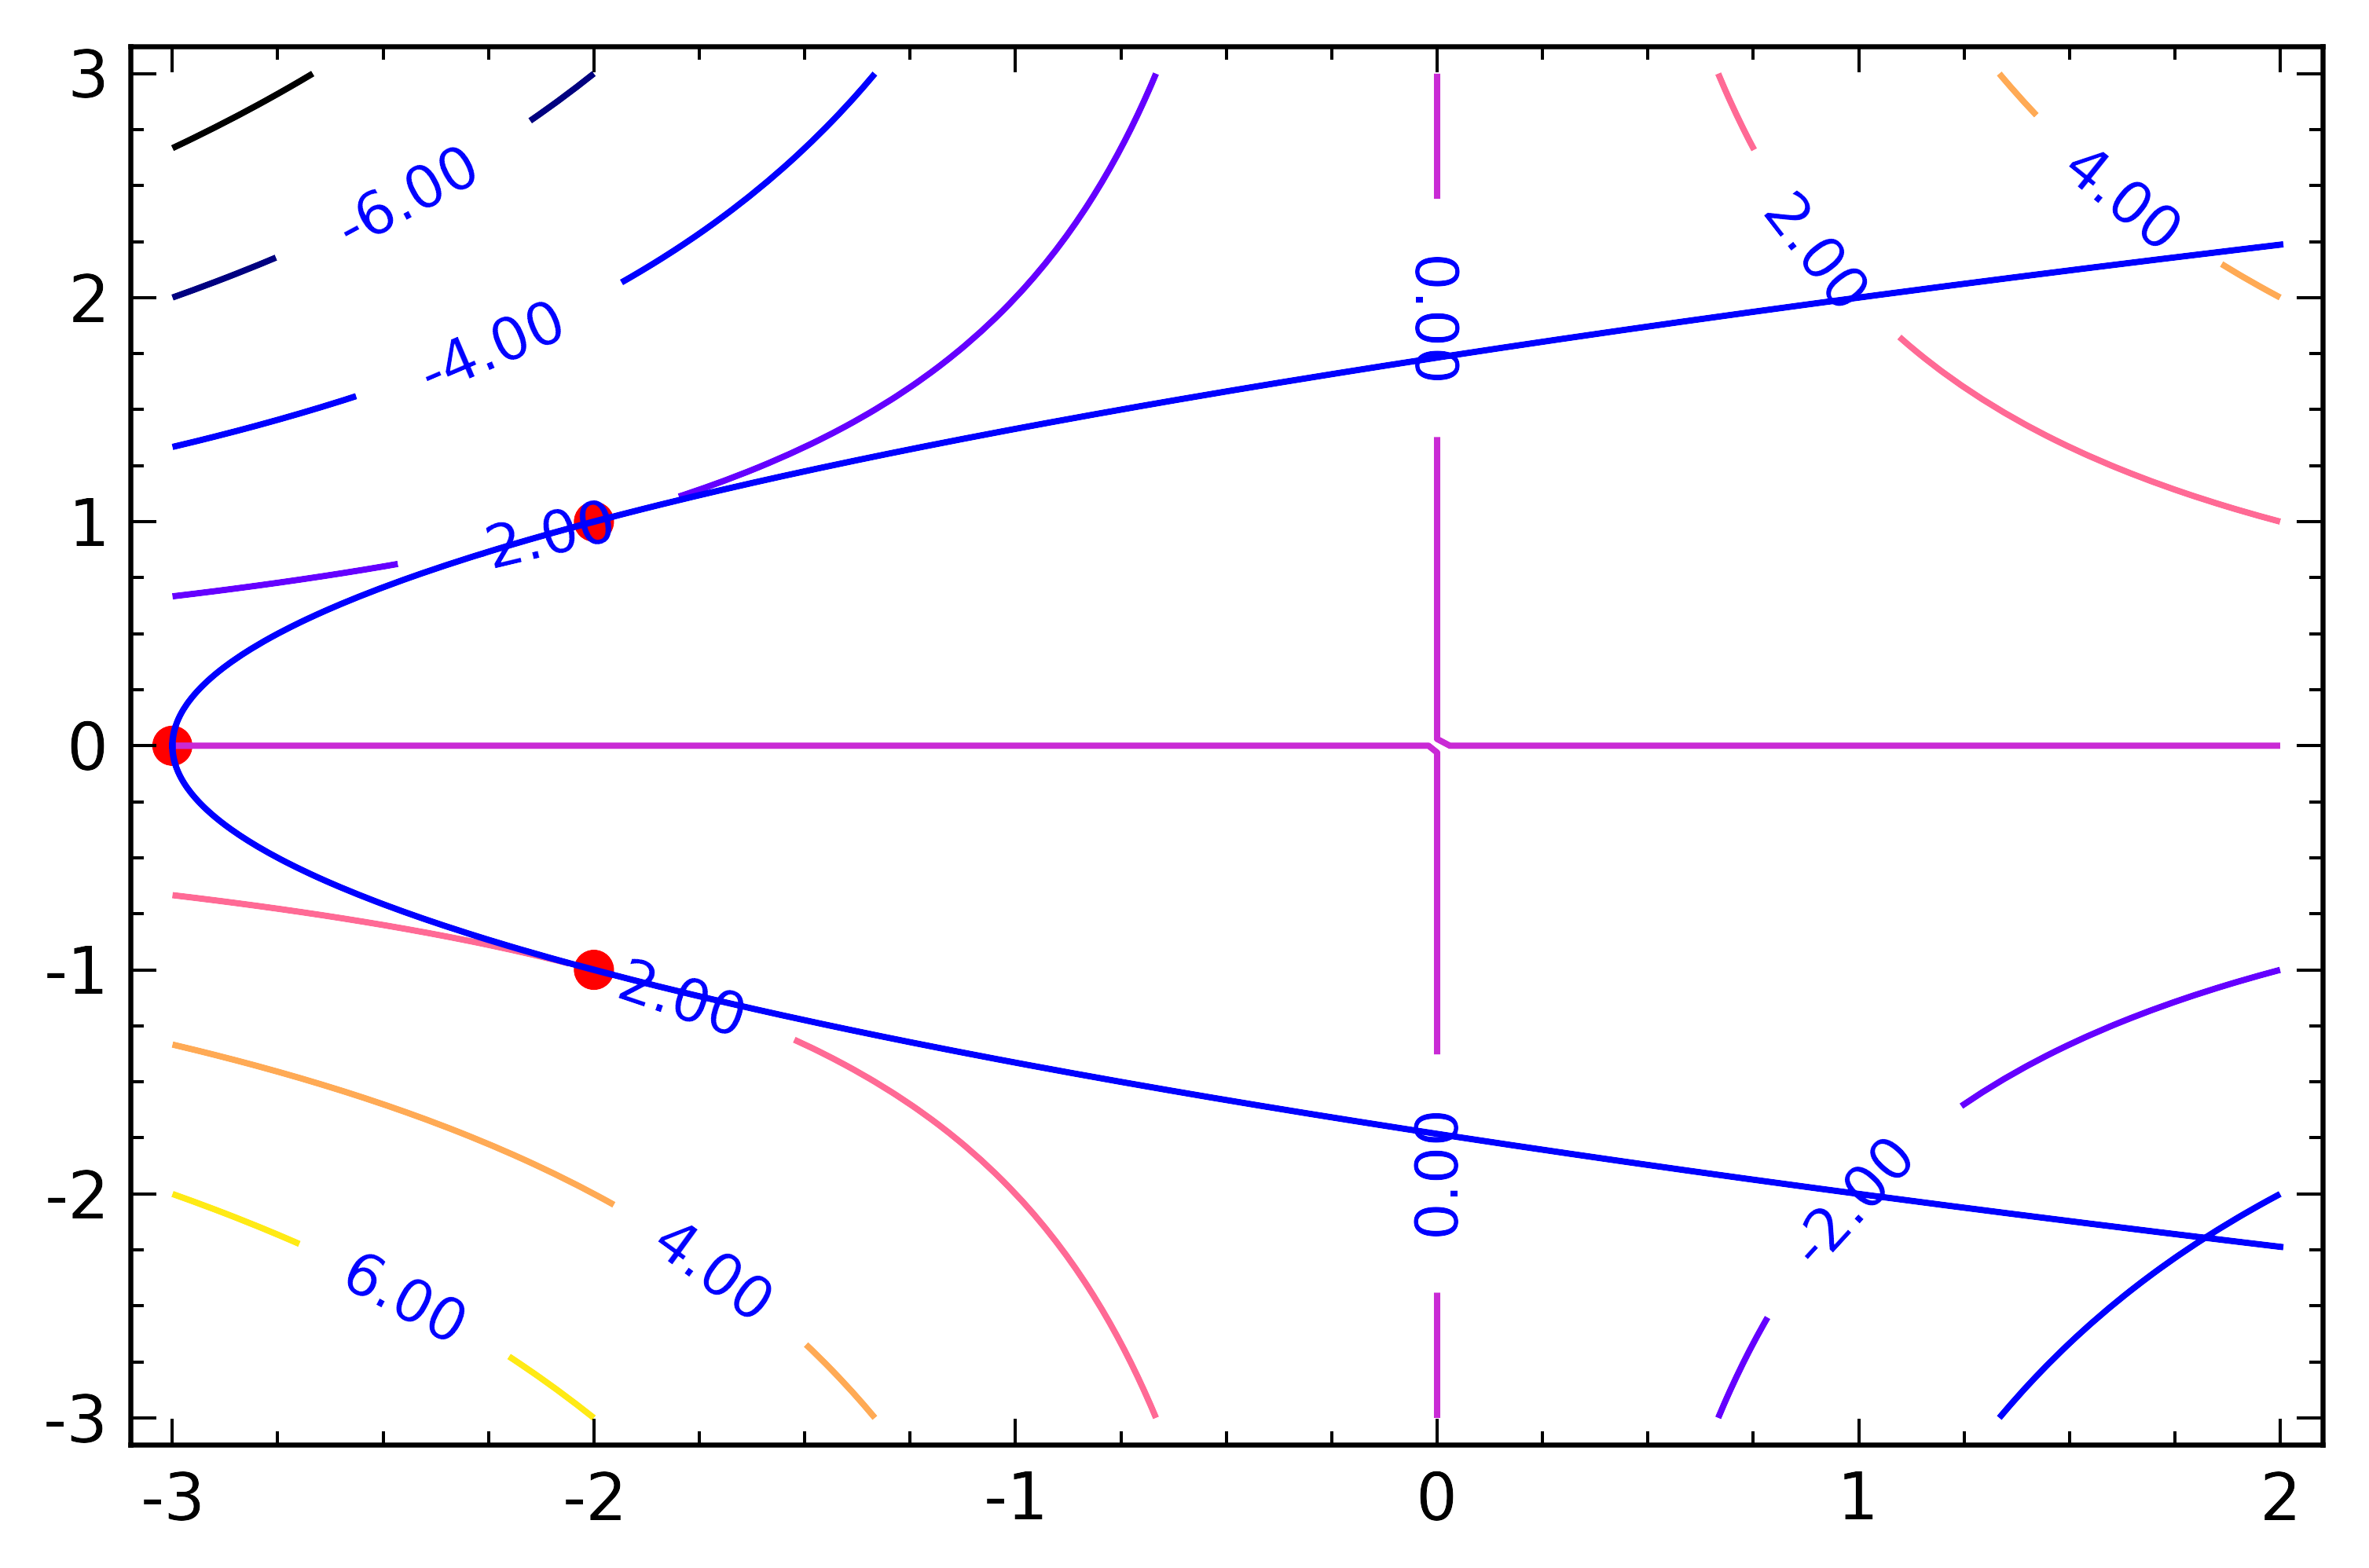
\includegraphics[scale=1]{kepek/kktkontur.png}
\end{center}

Globális minimuma pedig nem létezik a függvénynek, hiszen az $x_1$ tetszőlegesen nagy pozitív számnak, az $x_2$ pedig tetszőlegesen kicsi negatív számnak választható (természetesen csak a tartományon belül maradva), így az $f(x_1,x_2)=x_1x_2$ célfüggvény tetszőlegesen kis értéket vehet fel.
\end{megoldas}
